%todo: {Accuracy of Registration} improve the perception of the MR view via accurate registration. Anatomy learning, personal information (gender, age, body shape)
\section{User specific registration} \label{sec:3-PPMM:Registration}
The main advantage of the Magic Mirror framework is to create a personalized MR environment, which builds a link between the user's own body and the medical information. A personalized perception of the medical information is the major objective of the Magic Mirror, and it includes two parts: (i) correct medical information for current user and (ii) accurate registration of the non-physical visual effect. Registration is the most important part to forge an AR view of the user's body and a satisfactory non-physical visual effect.
The corresponding medical information is selected from the database, transformed to fit the user's body, and used to create a valid Magic Mirror effect (see \figurename{\ref{fig:3-MMC:MedicalInfoFlow}}). Via the color and depth camera, the system should detect the personal information (e.g., gender, age, height, etc.) to select the best medical information for the current user. 
However, the detection of personal information is mainly based on machine learning to calculate a general acceptable result. 
Hence, an interactive registration is introduced to improve the accuracy of the AR view.
In this section, personal information detection and interactive registration are discussed.

\subsection{Personal information detection}
%After a long time use of the Magic Mirror system in the real scenario, we figure out that the Magic Mirror framework is still imperfect. As the differences between children and adults, male and female, young and elders, the non-physical visual effect should be different. Sometimes the system has to be used under the supervision since some parameters of the user need to be input manually. It makes the using of the system limited without enough personal information. If it had more accurate personal information, better medical data would be selected and more satisfactory AR view would be generated.
To improve accuracy of the system framework, personal information, including gender, age, body size and pose of the user, should be collected. It can be implemented via biometric recognition, skeleton tracking, and 3D reconstruction. Then the corresponding medical volume is selected, transformed, and augmented onto the user body taking the collected personal information as parameters. 

\subsubsection{Personal information to collect}
If a new user is detected in the valid range of the system, the system goes to the stage of personal information detection and calculates all the parameters. The following list are the parameters we detect from each user.%, including gender, age, height, length of the limbs, 3D volume, weight, circumference, and body shape.
\begin{enumerate} [label=\arabic*.]
	\item  Gender: Define the sex of the user.
	\item Age: Classify into children, young, adult and elderly.
	\item  Height and length of limbs: Compute the height and limbs length of the user in millimeters.
	\item 3D volume: Reconstruct the 3D volume of the user. The volume is the upper part of the user's body.
	%as it is enough for the information extraction and the volume information of the legs and feet are not needed
	\item  Weight: Estimate the weight of the user.
	\item  Circumference: After obtain the upper part of the 3D volume, measure the circumference of the bust, waist and hip information of users.
	\item  Shape: Give the body shape information of the user in the WHR (waist-hip ratio) index.
\end{enumerate}

\subsubsection{System design}
\begin{figure}
	\centering
	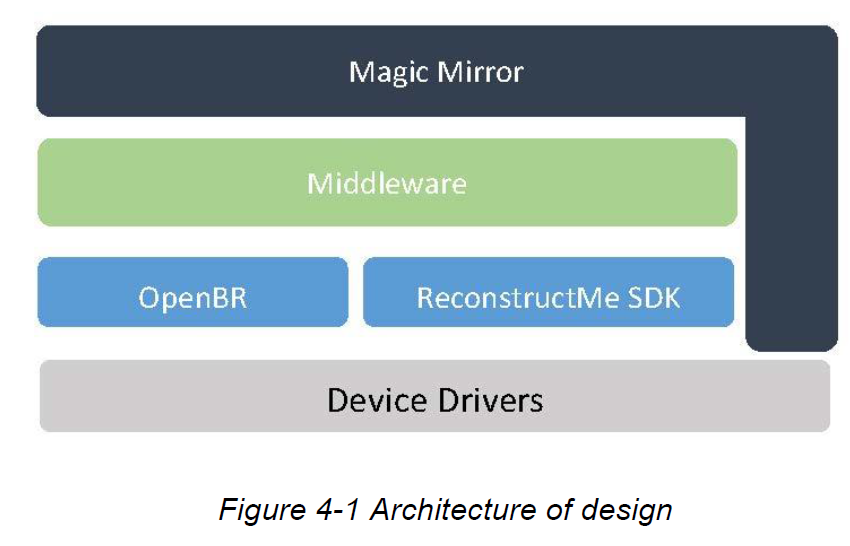
\includegraphics[width=0.7\linewidth]{figures/3-PRMM/middlewareFramework.png}
	\caption{Personal information collection. It is developed as a middleware, which works as an independent layer to collect the personal user information.}
	\label{fig:3-PRMM:middlewareFramework}
\end{figure}
The design of personal information collection is to develop a middleware, which works as an independent layer to collect the personal user information based on the color image, depth and skeleton stream from the Kinect sensor (see \figurename{\ref{fig:3-PRMM:InteractionWithMiddleware}}). An independent middleware would not affect the basic interaction of the Magic Mirror MR system. The middleware does not involve the non-physical visual effect definition. Through the whole processing of the user recognition, the middleware provides all the personal information of the user as parameters to the Magic Mirror AR view. All these parameters would help the system generate a better MR environment. 
%The middleware between the layer of hardware and the application of the Magic Mirror is an independent and automatic recognition procedure.

Once the middleware detects a user within the valid range of the system, it starts to collect the personal information of the user and the whole procedure of the iteration is described as \figurename{\ref{fig:3-PRMM:InteractionWithMiddleware}}.
The first step of using the middleware software is the same as the Magic Mirror system. The first task is user detection, to check if there is a new user in the view of the system. Then, the user is asked to stand straight in front of the system. When the user stands upright, the system detects the gender, age, height and limbs length. 
In the second step, the user needs to turn in a circle in front of the sensor in order to scan the user's body completely. When the user finishes this movement, the system would complete the collection of the personal user information. If the reconstruction fails, the system depicts a hint to repeat the whole process.
\begin{figure}
	\centering
	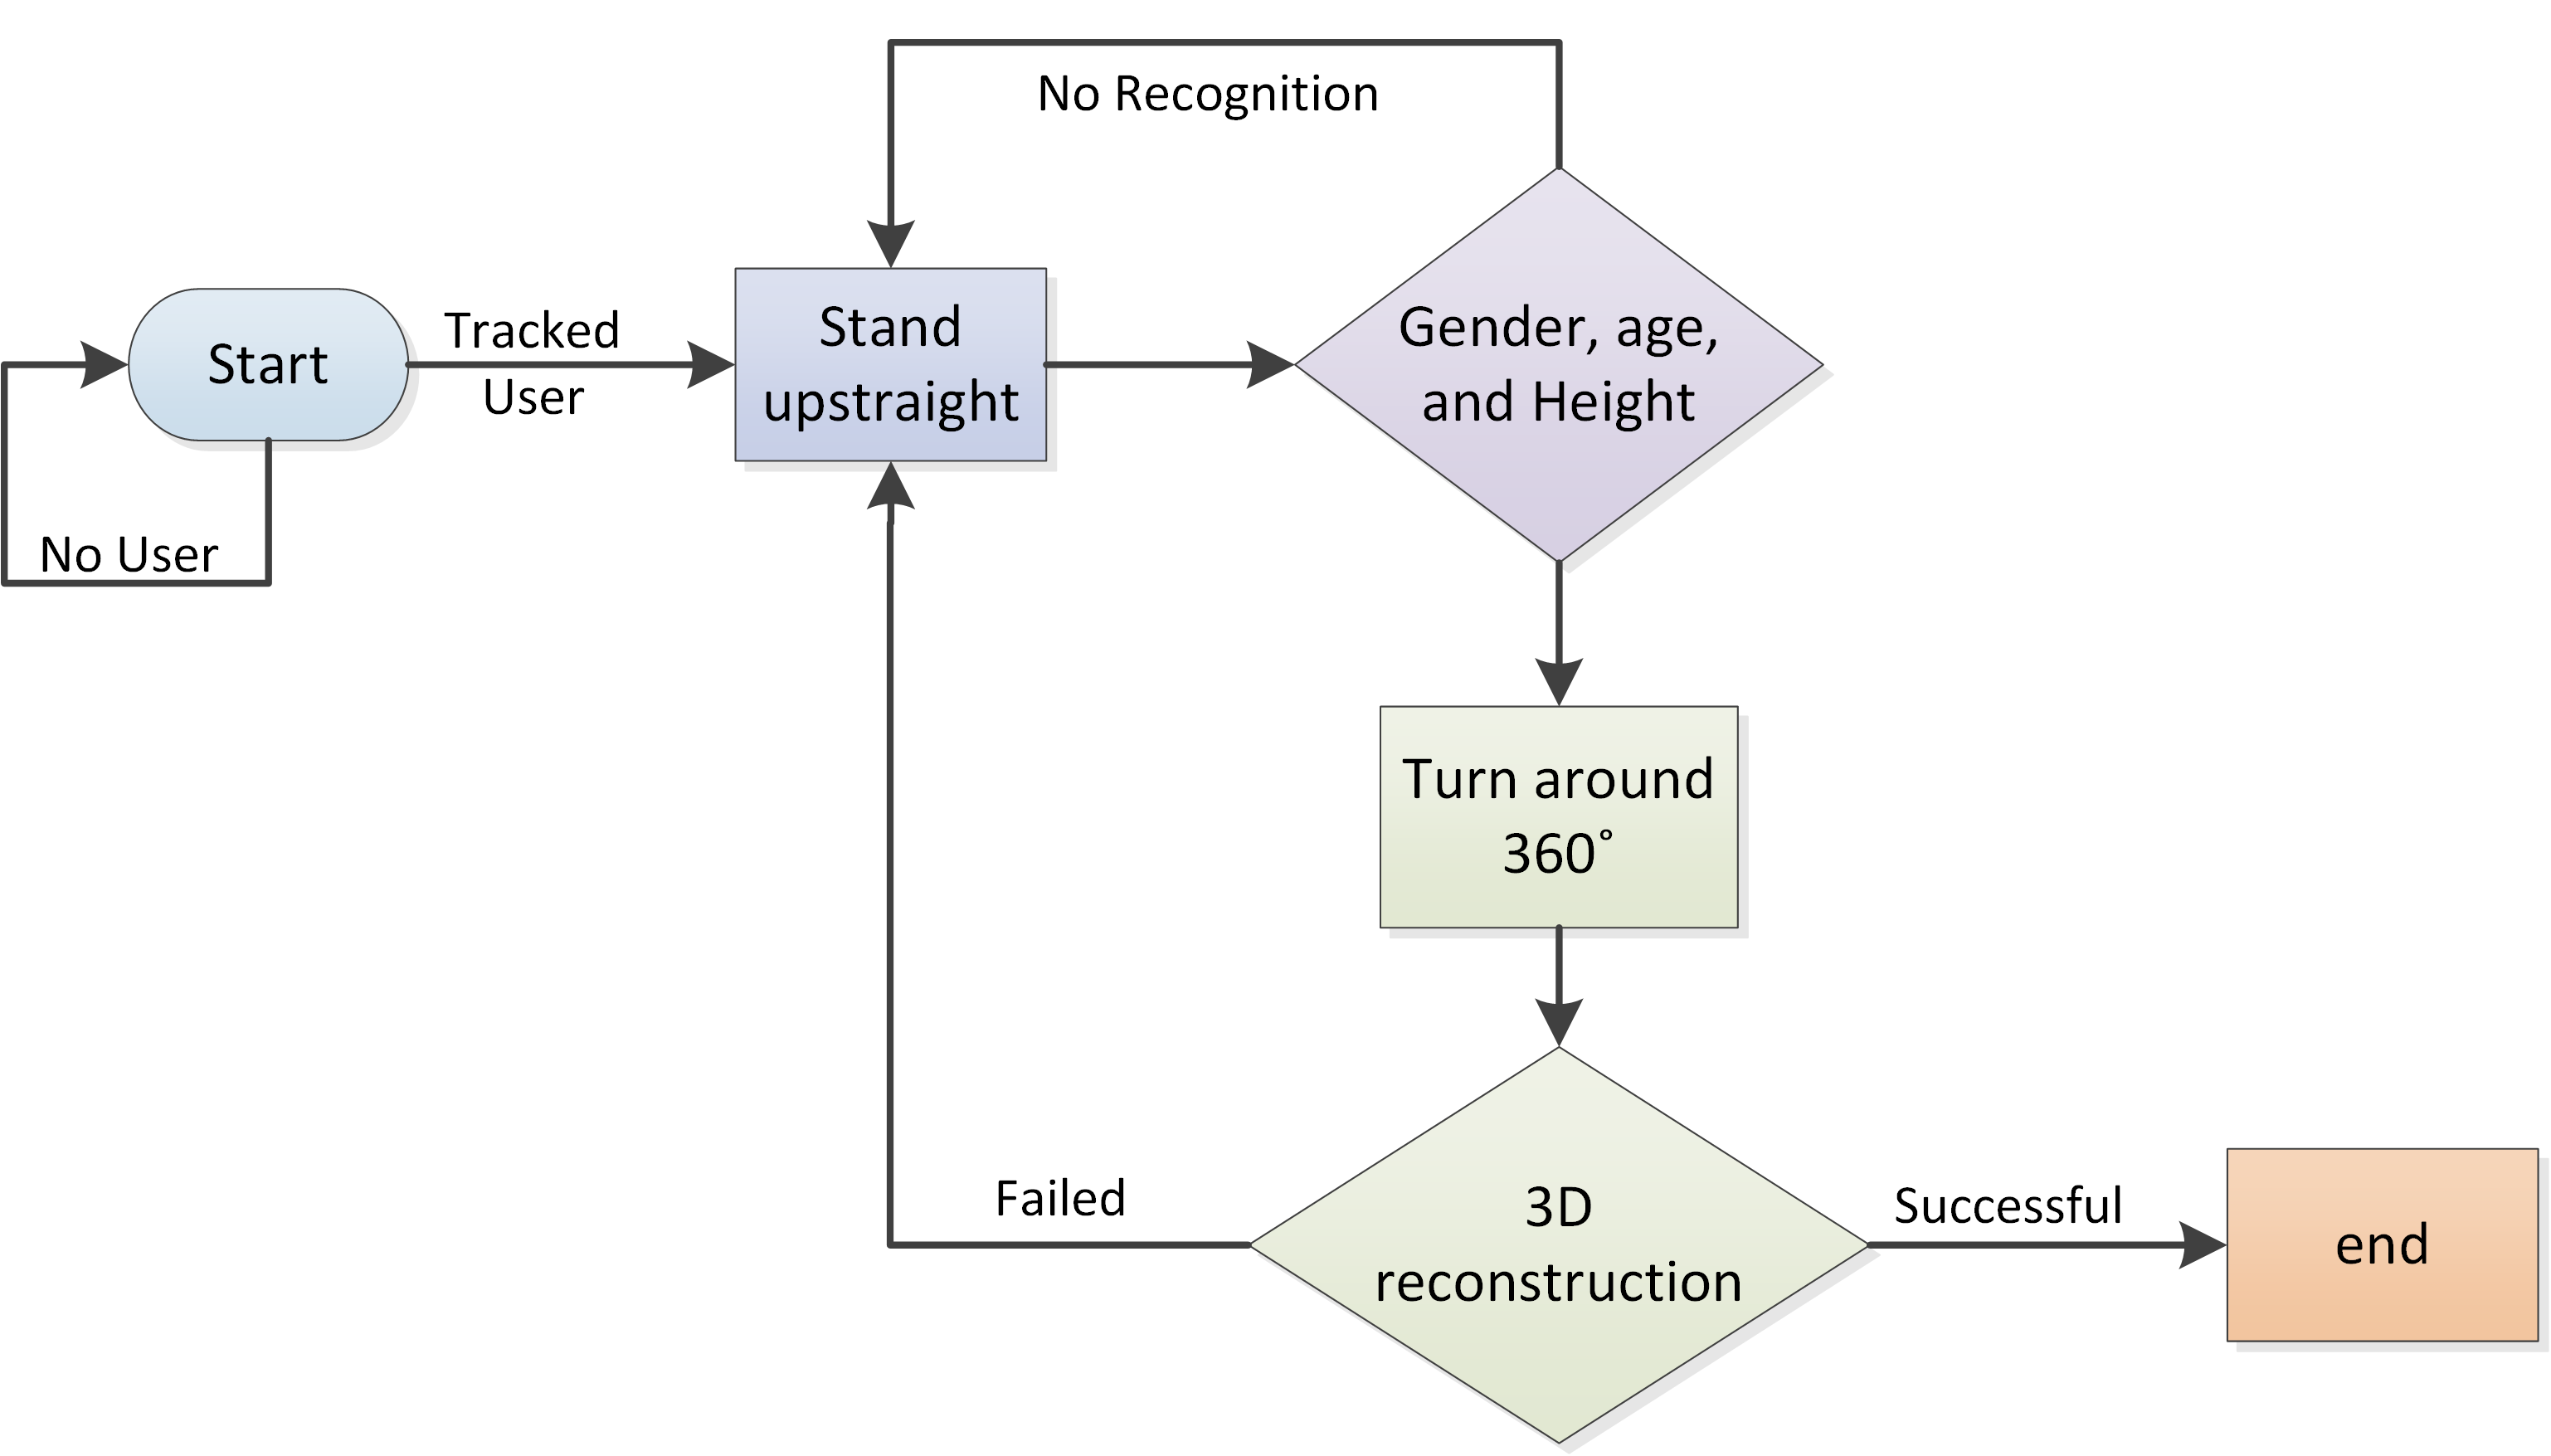
\includegraphics[width=0.75\linewidth]{figures/3-PRMM/InteractionWithMiddleware.png}
	\caption{Workflow of the interaction with the middleware to collect user personal information.}
	\label{fig:3-PRMM:InteractionWithMiddleware}
\end{figure}

\subsubsection{Implementation}
The color and depth cameras of the Kinect are the current sensors to observe the user and all the parameters of the user are detected via the color/depth images and the skeleton stream (see \figurename{\ref{fig:3-PRMM:BiomatricInformation}}). OpenBR framework is chosen to detect the gender and age from the captured color images. Meanwhile, the OpenNI and NITE libraries are adopted in this system for the height and limb length calculation. Besides the above parameters, weight, volume, circumference and body shape are all based on the 3D reconstruction of the user's upper body, which is done by the 3D reconstruction SDK and OpenCV\footnote{\url{http://opencv.org/}} libraries.
Combining all the following functions, the personal user information would be collected. The Magic Mirror framework can refer to the user's information as personalized parameters to generate more useful and interesting AR applications.
\begin{figure}
	\centering
	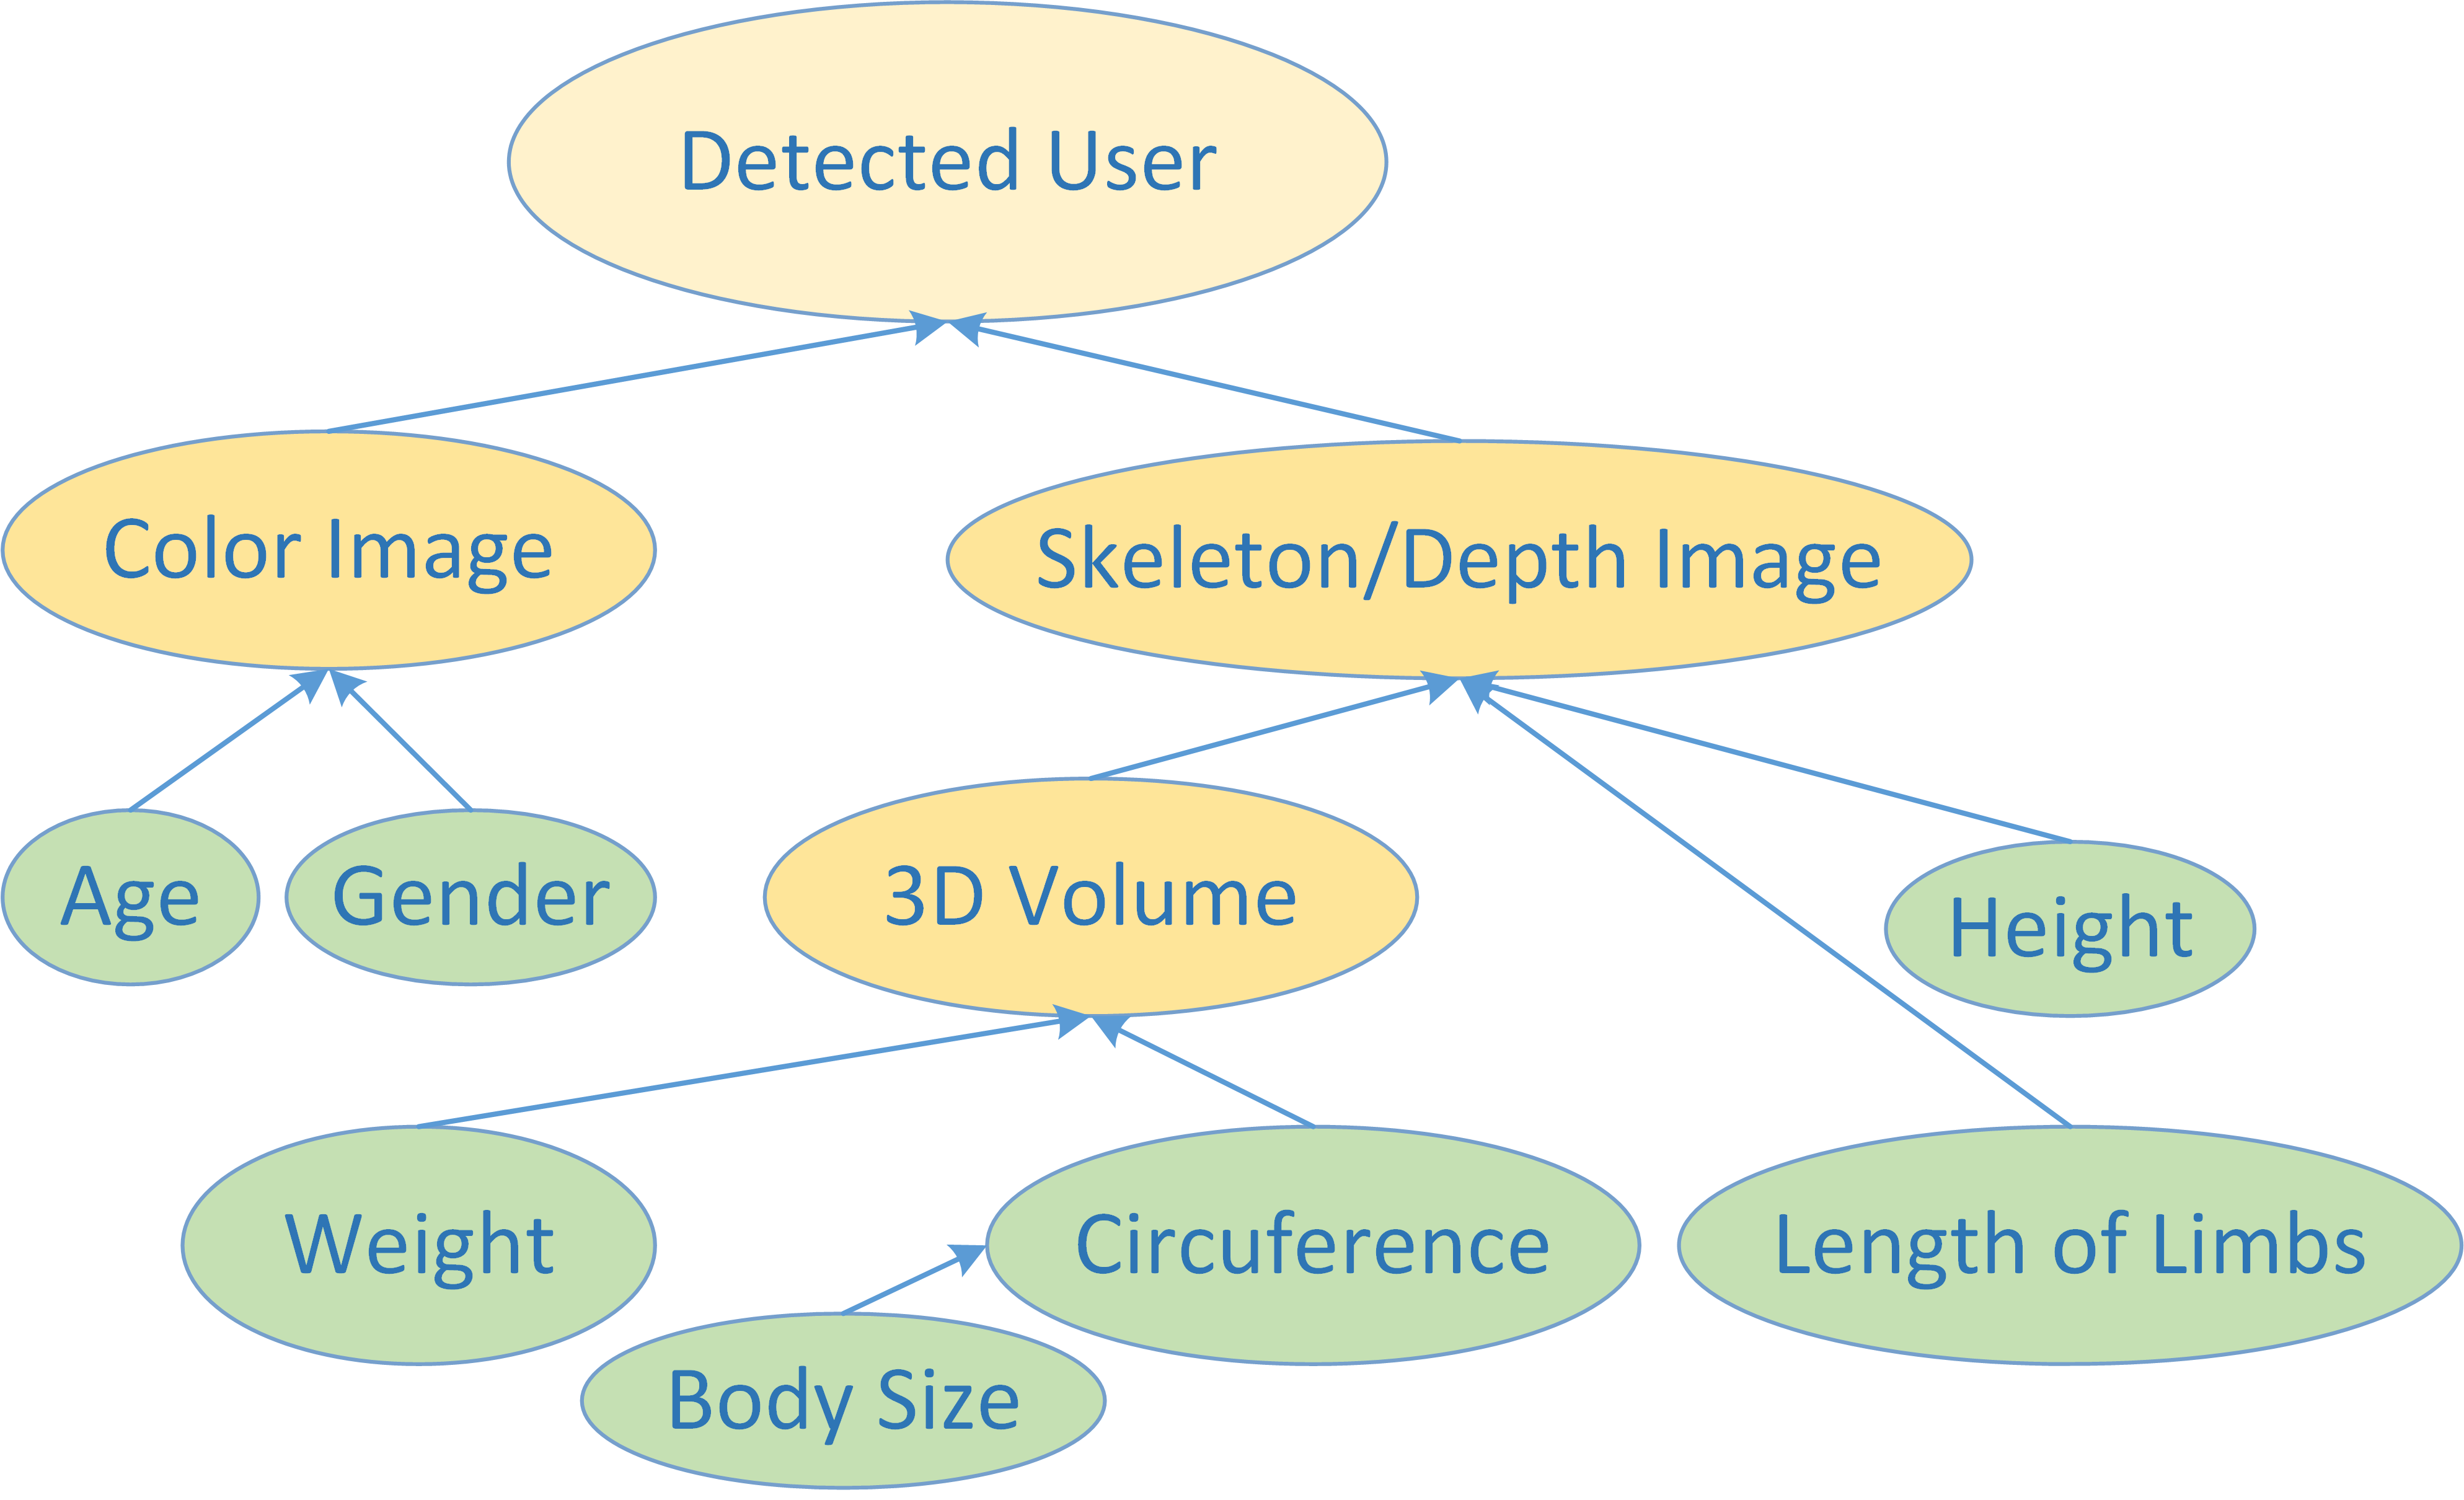
\includegraphics[width=0.75\linewidth]{figures/3-PRMM/BiomatricInformation}
	\caption{Personal information tree. All the parameters of the user personal information are detected via the color/depth images and the skeleton.}
	\label{fig:3-PRMM:BiomatricInformation}
\end{figure}

\paragraph{Gender and age}
The detection, normalization, representation and extraction are done by the OpenBR framework. What the middleware does is to implement a thread for this work. When a user stands in front of the system, the system firstly estimates the rotation of the human body. When the user faces the camera, an image is captured.  After the capturing, the image including the front face goes to the engine of the OpenBR framework, and then the gender and age are calculated. To get a more accurate result, a face area is selected based on the skeleton data. 

\paragraph{Height and length of limbs}
From the basic understanding of the word human height, we all know that the height is the distance from the top of the head to the bottom of the feet. 
As the feet sometimes may not be seen and detected by the Kinect sensor, the height would be converted to the distance from the top of the head to the ground.
Thanks to the help of the OpenNI and NITE SDK platform, the plane function of the floor could be easily assessed from the depth image and the user map is generated, defining the valid pixel belonging to the user's body in the depth image.
The coordinate of the top point of the user can be calculated, based on the user's information and the depth image. 
For the length of limbs, the user could be asked to keep a cross pose to get a clear view of the body and limbs. The limb length is the distances between corresponding skeleton joints.

\paragraph{3D volume}
The ReconstructMe framework is used to implement the 3D volume reconstruction.
% and the work-flow of the reconstruction is shown in \figurename{\ref{fig:3-PRMM:bodyReconstruction}}. 
One important task of the body reconstruction is to estimate the rotation angle of the user's body. If the total rotation angle of the user is less than $360\degree$, it means that the reconstruction is not finished and the system continues to reconstruct. The system tries to estimate the new position of the user, transforms the previous position to the new one and merges the data. After the transformation, it gets the next depth frame and repeats the reconstruction frame by frame until the sum of the angle changes is larger than 360 degree. %However, the procedure of the reconstruction would end if the tracking failed.
%\begin{figure}
%\centering
%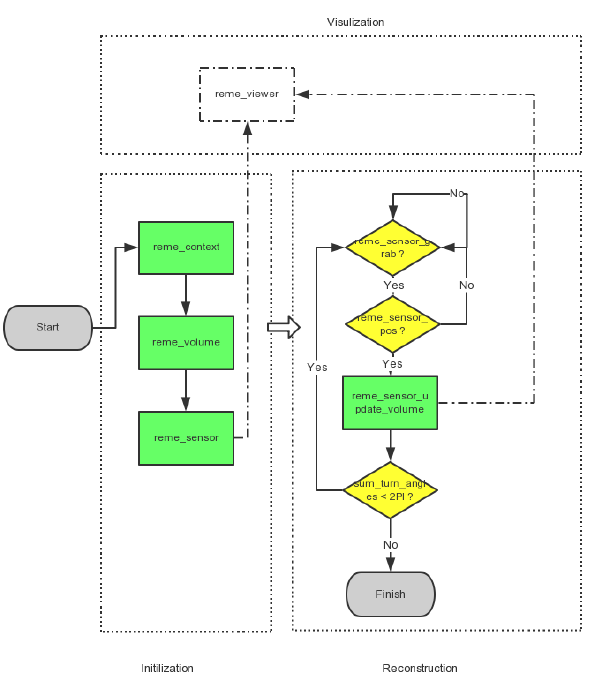
\includegraphics[width=0.7\linewidth]{figures/3-PRMM/bodyReconstruction}
%\caption{Flowchart of the reconstruction procedure}
%\label{fig:3-PRMM:bodyReconstruction}
%\end{figure}

\paragraph{Weight}
In the proposed middleware, we provide a simple method to estimate the weight information of the user. It is a simple idea that the weight is related to the volume of the 3D reconstruction. After the 3D reconstruction, a watertight 3D mesh is created and the volume is calculated \cite{Qiao2015}.
Due to the limitation of the Kinect sensor in the field of view, the 3D volume reconstructed cannot cover the whole body. However, we could just use the upper body of the user to estimate the full weight. As the result presented by \cite{Tozeren2000}, the upper body is about 68.2\% of the entire body weight. 
No matter how the reconstructed result is, the upper body is the volume without the part below the hip. As the hip joint information is known, we just make a cut from the hip position and generate a new volume without the hips.
As the density of human body is very near to the density of water ($1.0 g/cm^3$), the estimated weight of the user in the system would be as same as the volume.
\begin{equation}
Weight = (Volume * Density)/0.682
\end{equation}

\paragraph{Circumference and Body Shape}
After the obtainment of the 3D body volume of the user, the last measurement is to get the information of the user's shape like the circumference of bust, waist and hip. %The 3D volume is just a reconstructed model of the object and the further implementation is based on it.
From the reconstructed 3D volume, the body surface can be calculated easily. The circumference of the circle in each layer gives us the information of the user's body shape. As shown in \figurename{\ref{fig:3-PRMM:Circumference}}, it is a simple example of the user's body when we look at the volume in the middle layer from the cross-sectional view. The blue circle is the Z axis cut on the 3D volume and the length of the cut would refer to the circumference on that layer.
\begin{figure}
	\centering
	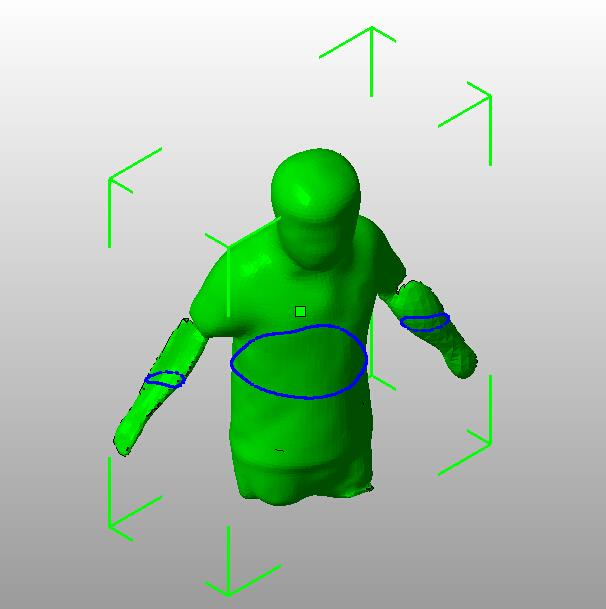
\includegraphics[width=0.5\linewidth]{figures/3-PRMM/Circumference}
	\caption{Circumference. The circumference of the circle in each layer in the 3D body volume gives us the information of the user's body shape.}
	\label{fig:3-PRMM:Circumference}
\end{figure}
The key point here for the body shape detection is how to find the right layer for the right circle we want. The bust, waist and hip are the most important parameters for the body shape detection within the system. 
The position of the bust, waist and hip can be estimated from the skeleton, we can refer to the correspondent layer of them and acquire the length of each parameters.
%Right now, for the bust, waist and hip detection, the neck joint, torso joint and hip joint are under consideration.
%The circumference in the shoulder joint is the shoulder circumference. As the same idea, the bust is in the middle between the shoulder and torso. The waist is in the middle between the torso and hip. The hip is the layer refer the position of the hip joint as well.
Body shape information of the user refers to the index of health and the risk of developing serious health conditions. The Waist-Hip-Ratio (WHR)\cite{Consultation2008} is introduced to indicate the condition of obesity for the system's users. The ``apple shaped'' bodies would be more healthy than the ``pear shaped'' as less weight around the waist makes the value of WHR smaller.
The system would provide the value of Waist-Hip-Ratio index to the user and indicate the health condition of them.

\subsection{Interactive registration}
The skeleton output from Kinect also limits the precision of the Magic Mirror applications. Thus, the Magic Mirror augmentations would contain errors and users would easily distinguish anatomical offsets on their body resulting in a poor mixed reality environment and visualization. Alternatively, we considered projectors to display human anatomy and along with their existing limitations the same inaccuracies would exist \cite{Sun2013}. 
Hence, an interactive solution is proposed to improve the registration as the Magic Mirror framework always takes the user movement as input.
Our aim is then to propose a method to correct for such overlay inaccuracies that can be used in the general Magic Mirror framework. 

\subsubsection{Anatomical bone landmarks}
Together with orthopedic surgeons, we have defined five bone landmarks that (i) users can easily identify and touch while standing in front of the Kinect, and (ii) that are accurately and easily identified in medical data such as CT \cite{ma2013ismar}. These are: left and right acromion, left and right anterior superior iliac spine, and the manubrium (see \figurename{\ref{fig:3-PRMM:bonelandmarker}}).
\begin{figure}[htb]
	\centering
	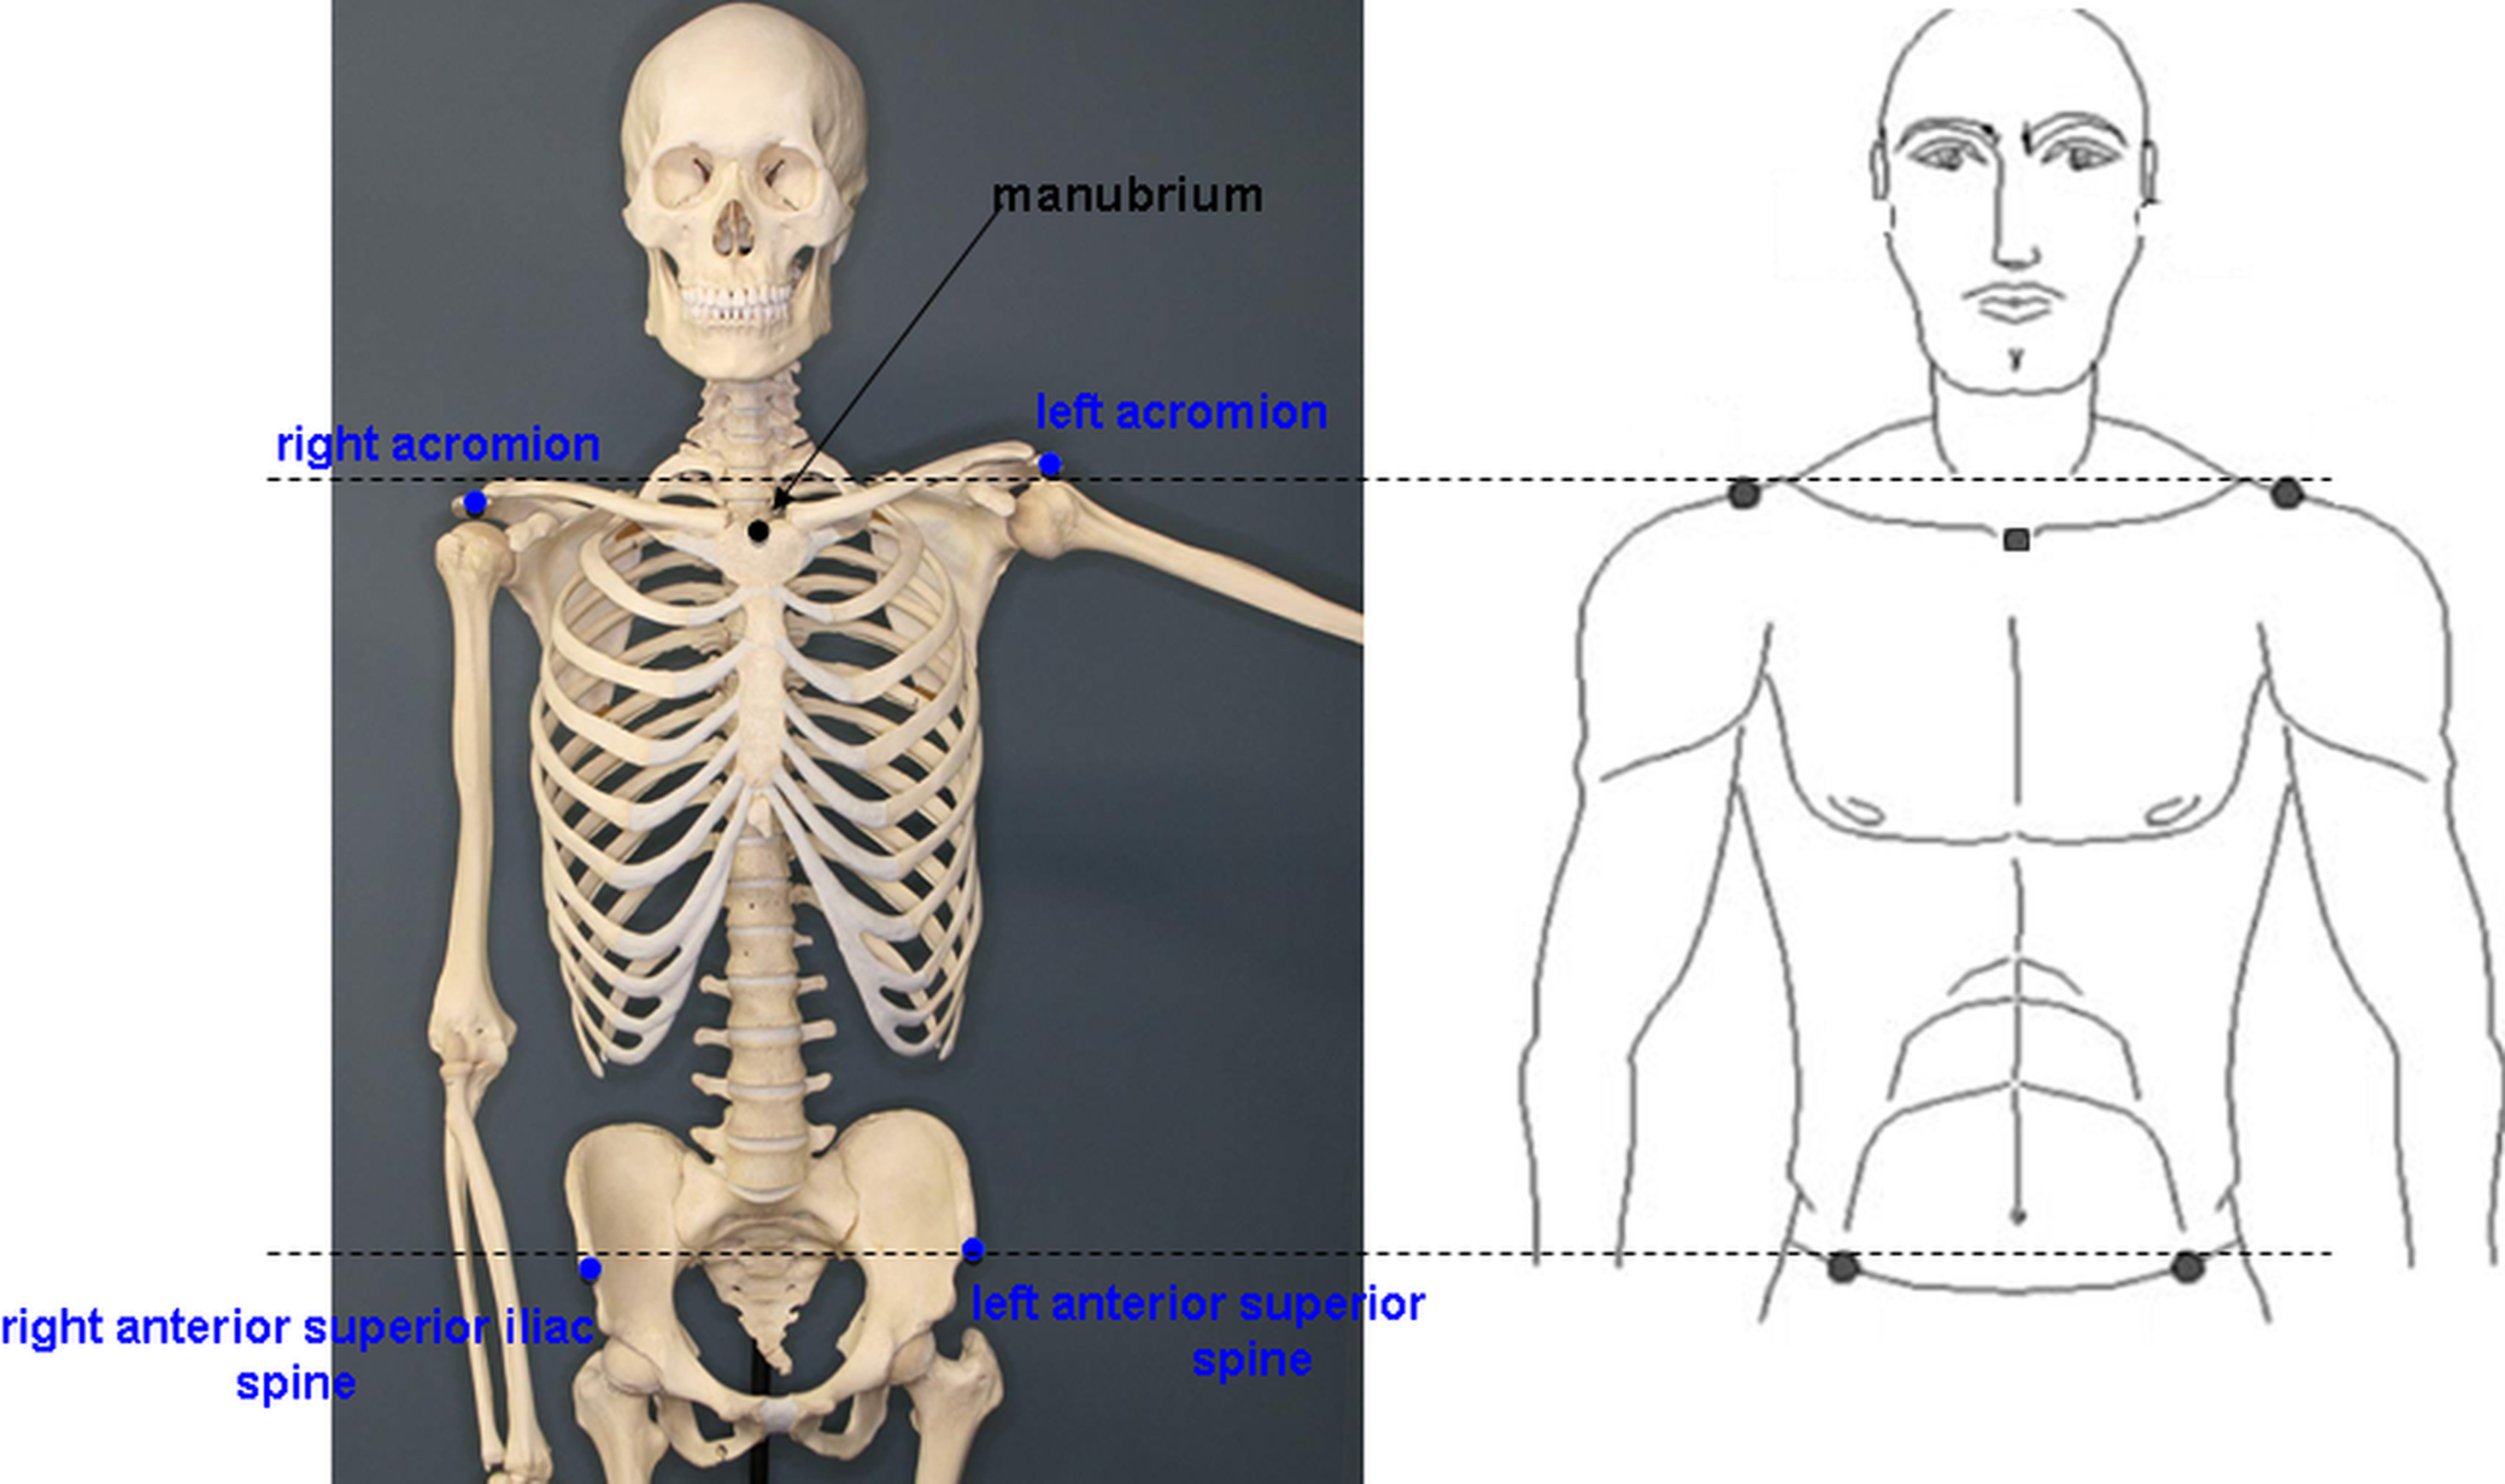
\includegraphics[width = \linewidth]{figures/3-PRMM/FiveBoneLandmarker.png}
	\caption{Anatomical bone landmarks. Selected anatomical points for Kinect skeleton improvement and subsequent CT warping and interpolation.}
	\label{fig:3-PRMM:bonelandmarker}
\end{figure}

Prior to correctly using the Magic Mirror system, the users stand in front of the monitor and virtual marks are displayed near the five bone landmarks according to the raw skeleton stream. The users are asked to interactively adjust the positions of the five marks to fit their own bone positions. In addition, the exact locations in the VKH CT dataset of the five selected bone landmarks are known. A linear interpolation was executed to estimate the torso point (i.e. a $6^{th}$ landmark) in the CT volume to improve the overlay. Then the scale factors and transformation matrix were computed to render the anatomical image onto the user's body. These landmark positions allow the deformation and interpolation of the medical data correctly within the Magic Mirror and onto the human body, resulting in a more precise augmentation. A user study involving surgeons and anatomy experts confirmed our findings and will be presented in the following section.
%%%%%%%%%%%%%

%tranditional way to do the registration
\subsubsection{Improvement of Kinect skeleton}
We present a general method to interactively improve and correct the Kinect skeleton for anatomy education purposes. The method can also be applied to projectors or other sensors as well as for general augmented reality applications. A thorough validation of our method demonstrated improved precision of anatomical landmarks and opens the avenue to future improvements in medical education. 
\figurename{\ref{fig:3-PRMM:5Joints}} shows a comparison between the traditional Kinect skeleton and its proposed improvement. The first row depicts visually the exactness of the new skeleton. The second row depicts the skeleton landmarks directly on CT data. We observe that the shoulder and anterior superior spine are inaccurate in the images. The last row depicts the selected bone landmark positions within CT as well. Transverse and sagittal CT slices of the visible human Korean are seen respectively in rows 2 and 3.

\paragraph{Normal solution} To improve the perception of the AR view, the medical data has to be registered to the current user. A simple method used by the Magic Mirror framework is that an orthopedic clinician helps to find the corresponding Kinect skeleton joints in the CT volume (see \figurename{\ref{fig:3-PRMM:5Joints:a}} and \figurename{\ref{fig:3-PRMM:5Joints:c}}). The points 1-5 are raw Kinect skeleton joints and slices 1-5 are estimated by the clinician according to the yellow line drawn on user's body using the raw Kinect skeleton joints information. So the scaling factor from CT volume to the current user is:
\begin{equation}
	WidthScale = Avg(\frac{{{W_{12}}}}{{W_{12}^{CT}}},\frac{{{W_{34}}}}{{W_{34}^{CT}}})
\end{equation}
\begin{equation}
	HeightScale = Avg(\frac{{{H_{14}}}}{{H_{14}^{CT}}},\frac{{{H_{23}}}}{{H_{23}^{CT}}})
\end{equation}
$T_{K\_CT}$ is the transformation from Kinect coordinate system to CT volume. $T_{K\_n}$ and $T_{CT\_n}$ is the transformation matrix from the original point in Kinect world and CT volume to the skeleton joint $n$, correspondingly.
\begin{equation}
	T_{K\_CT} = T_{K\_5} * T_{CT\_5}.inv()
\end{equation}
\begin{figure} 
	\centering
	\subfloat[~Kinect skeleton]{ \label{fig:3-PRMM:5Joints:a}
		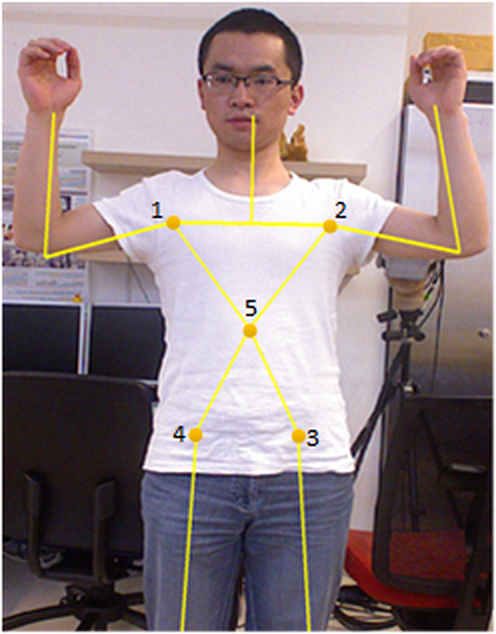
\includegraphics[height = 8.5cm]{figures/3-PRMM/Kinect5Joints.png}
	}
	\quad
	\subfloat[~Improvement of Kinect skeleton]{ \label{fig:3-PRMM:5Joints:b}
		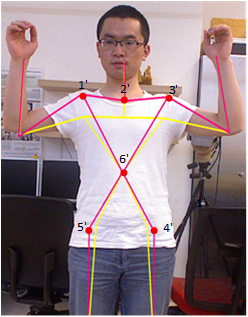
\includegraphics[height = 8.5cm]{figures/3-PRMM/Kinect6Joints.png}
	}
	\quad
	\subfloat[~Skeleton joints in CT volume]{ \label{fig:3-PRMM:5Joints:c}
		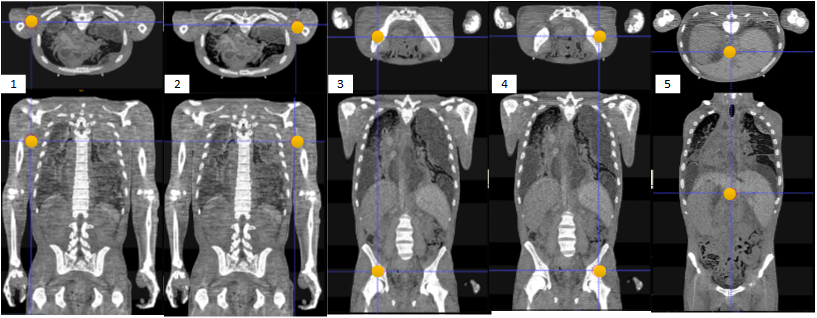
\includegraphics[width = \linewidth]{figures/3-PRMM/Kinect5JointsCT.png}
	}
	\quad
	\subfloat[~Bone landmarks in CT volume]{ \label{fig:3-PRMM:5Joints:d}
		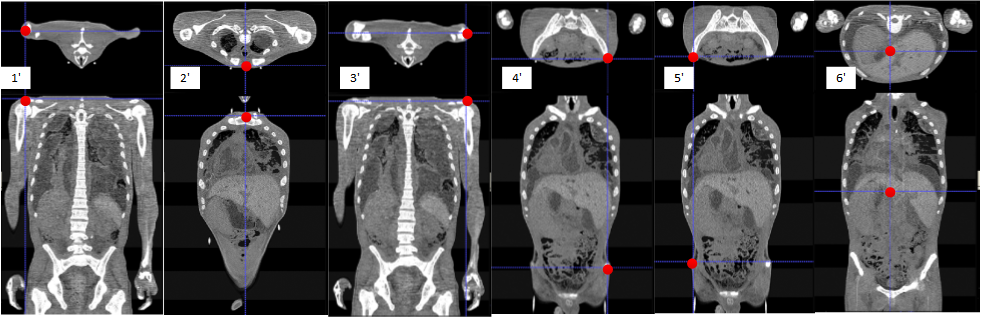
\includegraphics[width = \linewidth]{figures/3-PRMM/Kinect6JointsCT.png}
	}
	\caption{The inaccurate Kinect skeleton (a) The points 1-5 are raw Kinect skeleton joints. (b) The inaccurate Kinect skeleton, in yellow, compared to the improved Kinect skeleton positions in red. The points 1'-5' are the position of the five selected bones, which are suggested by orthopedic clinicians. (c) Slices 1-5 are estimates by  orthopedic clinicians according to the yellow line drawn on the user's body using the Kinect skeleton joints information. (d) Slices 1'-5' are the selected five bones suggested by orthopedic clinicians and the slice 6', which is computed from slice1'-5', is the corresponding slice for joint 6'.}
	\label{fig:3-PRMM:5Joints}
\end{figure} 
\paragraph{Proposed method} The goal of the proposed method is to create a more precise user-specific AR overlay environment. The positions of the anatomical bone landmarks can improve the deformation and interpolation of the medical data, resulting in a more precise Kinect skeleton and augmentation. The following scale factors were calculated for the improved system via the selection of bone landmarks. 
\begin{equation}
WidthScale = Avg(\frac{{{W_{1'3'}}}}{{W_{1'3'}^{CT}}},\frac{{{W_{4'5'}}}}{{W_{4'5'}^{CT}}})
\end{equation}
\begin{equation}
HeightScale = Avg(\frac{{{H_{1'5'}}}}{{H_{1'5'}^{CT}}},\frac{{{H_{3'4'}}}}{{H_{3'4'}^{CT}}},\frac{{{H_{2'4'}}}}{{H_{2'4'}^{CT}}})
\end{equation}
$T_{K\_n'}$ and $T_{CT\_n'}$ is the transformation matrix from the original point in Kinect world and CT volume to the bone marker $n'$, correspondingly. Using Eq.\ref{eq:3-PMRR:6CT}, the position of the torso in the CT volume is calculated. The transformation of the torso is the linear interpolation of the five bone landmarks.
\begin{equation} \label{eq:3-PMRR:6CT}
T_{CT\_6'} = Avg(T_{CT\_n'} * T_{K\_n'}.inv() * T_{K\_5 })
\end{equation}
\begin{equation}
T_{K\_CT'} = T_{K\_6'} * T_{CT\_6'}.inv()
\end{equation}

\subsubsection{Evaluation}
As an augmented reality anatomy learning application, both accuracy and system usability are very important prior to its translation into the classroom. We undertook one user study with particular users having expert anatomy knowledge to evaluate if this system is precise enough for anatomy learning.% and the proposed method improves the accuracy of the AR view.

\paragraph{Assessing the Magic Mirror system precision and usability}
Participants: Seven participants were included in this study (two surgeons and five final year undergraduate medical students). 
Analysis: a Likert scale was used which is a type of psychometric response scale often used in surveys and the most widely used scale in survey research. When responding to a Likert questionnaire item, respondents specify their level of agreement to a statement. The format of our 5-pt Likert was: (1) \textit{strongly disagree}, (2) \textit{disagree}, (3) \textit{neither agree nor disagree}, (4) \textit{agree}, (5) \textit{strongly agree}. 

To assess the precision of our personalized Magic Mirror we asked the participants to interact with the system platform which integrates user-specific anatomical landmark selection. Participants were asked to provide an estimated numerical offset, if any, on how far specific bone landmarks or organs were with respect to their own body. For this, they interacted with the Magic Mirror window, CT data, and used their own medical knowledge and expertise for judgment. CT data was displayed in an interface depicting both transverse and sagittal planes, and participants would quantify the offsets. If needed, a ruler was provided to assist them. The anatomical targets during evaluation were defined as: the anterior superior iliac spine, manubrium, heart, and liver. 
Results from this exercise are shown in \tablename{\ref{tb:3-PRMM:results1}}, with offsets measured in centimeters.  The user study showed the impact of the proposed method to increase precision for a better visualization of anatomy. The offsets of specific anatomical landmarks decreased significantly. Results from the user study show that the precision of the user-specific learning environment is on average 0.96cm.
\begin{table}
	\caption{Precision (in cm) of magic mirror system based on anatomical offsets}
	\label{tb:3-PRMM:results1}
	\scriptsize
	\begin{center}
		\begin{tabular}{p{4cm}|p{3cm}}
			Anatomy & Offset(Mean$\pm$ STDev) \\
			\hline
			anterior superior iliac spine & $0.67\pm0.52$\\
			manubrium & $0.67\pm0.75$ \\
			heart & $1.17\pm1.60$\\
			liver & $1.33\pm1.21$
		\end{tabular}
	\end{center}
\end{table}

The seven participants were then asked to judge the usability of the AR Magic Mirror system by responding to the following questions: (i) is the overlay accurate w.r.t human body (ii) is the user interface easy to use, (iii) is it fun to play, (iv) can it be used for medical education, and (v) would it have stronger impact for medical education learning?
The Likert scale results for the first four questions are shown in \tablename{\ref{tb:3-PRMM:results2}}.
\begin{table}
	\caption{Likert scale results regarding magic mirror usability}
	\label{tb:3-PRMM:results2}
	\scriptsize
	\begin{center}
		\begin{tabular}{p{8cm}|p{3cm}}
			\space & Mean$\pm$ STDev \\
			\hline
			is the augmented reality overlay accurate w.r.t human body & $4.00\pm0.89$\\
			is the user interface easy to use & $3.67\pm1.03$ \\
			is it fun to play & $4.50\pm0.55$\\
			can it be used for medical education & $4.17\pm0.75$
		\end{tabular}
	\end{center}
\end{table}

For the last question regarding the impact of our technology, there was a unanimous response that the AR Magic Mirror system should be considered as a potential platform to complement existing anatomy learning tools inside anatomy classrooms. 

\subsubsection{Conclusion}
%todo conclution and discussion with the first part.
The precision of our method is visually demonstrated in \figurename{\ref{fig:3-PRMM:ResComparing}}. We observe that the acromion and anterior superior iliac spine, using the traditional Kinect skeleton, is not positioned correctly within the CT data compared to the modified Kinect skeleton version (1-2 vs. 1'-2'; 3-4 vs. 3'-4'). The orthopedic surgeons participating in our study confirmed this.
\begin{figure}[htb]
	\centering
	\includegraphics[width = \linewidth]{figures/3-PRMM/ResComparing.png}
	\caption{The Magic Mirror before (top) and after (bottom) the Kinect skeleton adjustment. Column 2 depicts the bottom of the rib cage being positioned correctly after skeleton correction.}
	\label{fig:3-PRMM:ResComparing}
\end{figure}
Results from a user study show the impact of interactively improving the Kinect skeleton to increase precision for a better visualization of anatomy. The offsets of specific anatomical landmarks decreased significantly. The following comments were also collected from the user study:
\begin{enumerate}
	\item the precision improved; making the user touch anatomical landmarks is cool since this is the way it is done in clinic …
	\item two additional landmarks easily accessible are the sternum and bottom of rib cage…
	\item make the Magic Mirror circle bigger for larger anatomy …
	\item voice command is a good idea but it is sensitive to the surroundings noise (i.e. multiple people talking in the room, etc.)
	\item interactions between observers …
	\item could introduce the female CT visible human Korean …
	\item could use a healthy patient CT or other modality …
	\item could make the CT slices bigger on the screen …
\end{enumerate}

This section presented a general method to collect the personal information and interactively improve and correct the Kinect skeleton for anatomy education purposes. 
%We believe that our general method can be applied to projectors or other sensors as well for augmented reality. 
A thorough validation of our method demonstrated improved precision of anatomical landmarks and opens the avenue to future improvements in medical education.